\documentclass{article}
\usepackage[utf8]{inputenc}
\usepackage{geometry}
\usepackage{graphicx}
\graphicspath{./images/}
\usepackage{subcaption}
\geometry{
    margin=1in,
    top=10mm,
}

\title{Reinforcement Learning CW1}
\author{Taixi Pan}
\date{November 2022}

\begin{document}

    \maketitle


    \section{Question 1}\label{sec:question-1}

    \subsection{Part 1}\label{subsec:question-1-1}
    I used value iteration to implement the DP agent.
    Value iteration is chosen to allow for more efficient computation without losing the convergence property, as it only involves one iteration of policy evaluation instead of a full one.

    \subsection{Part 2}\label{subsec:question-1-2}

    \begin{figure}[h]
        \begin{subfigure} {0.5\textwidth}
            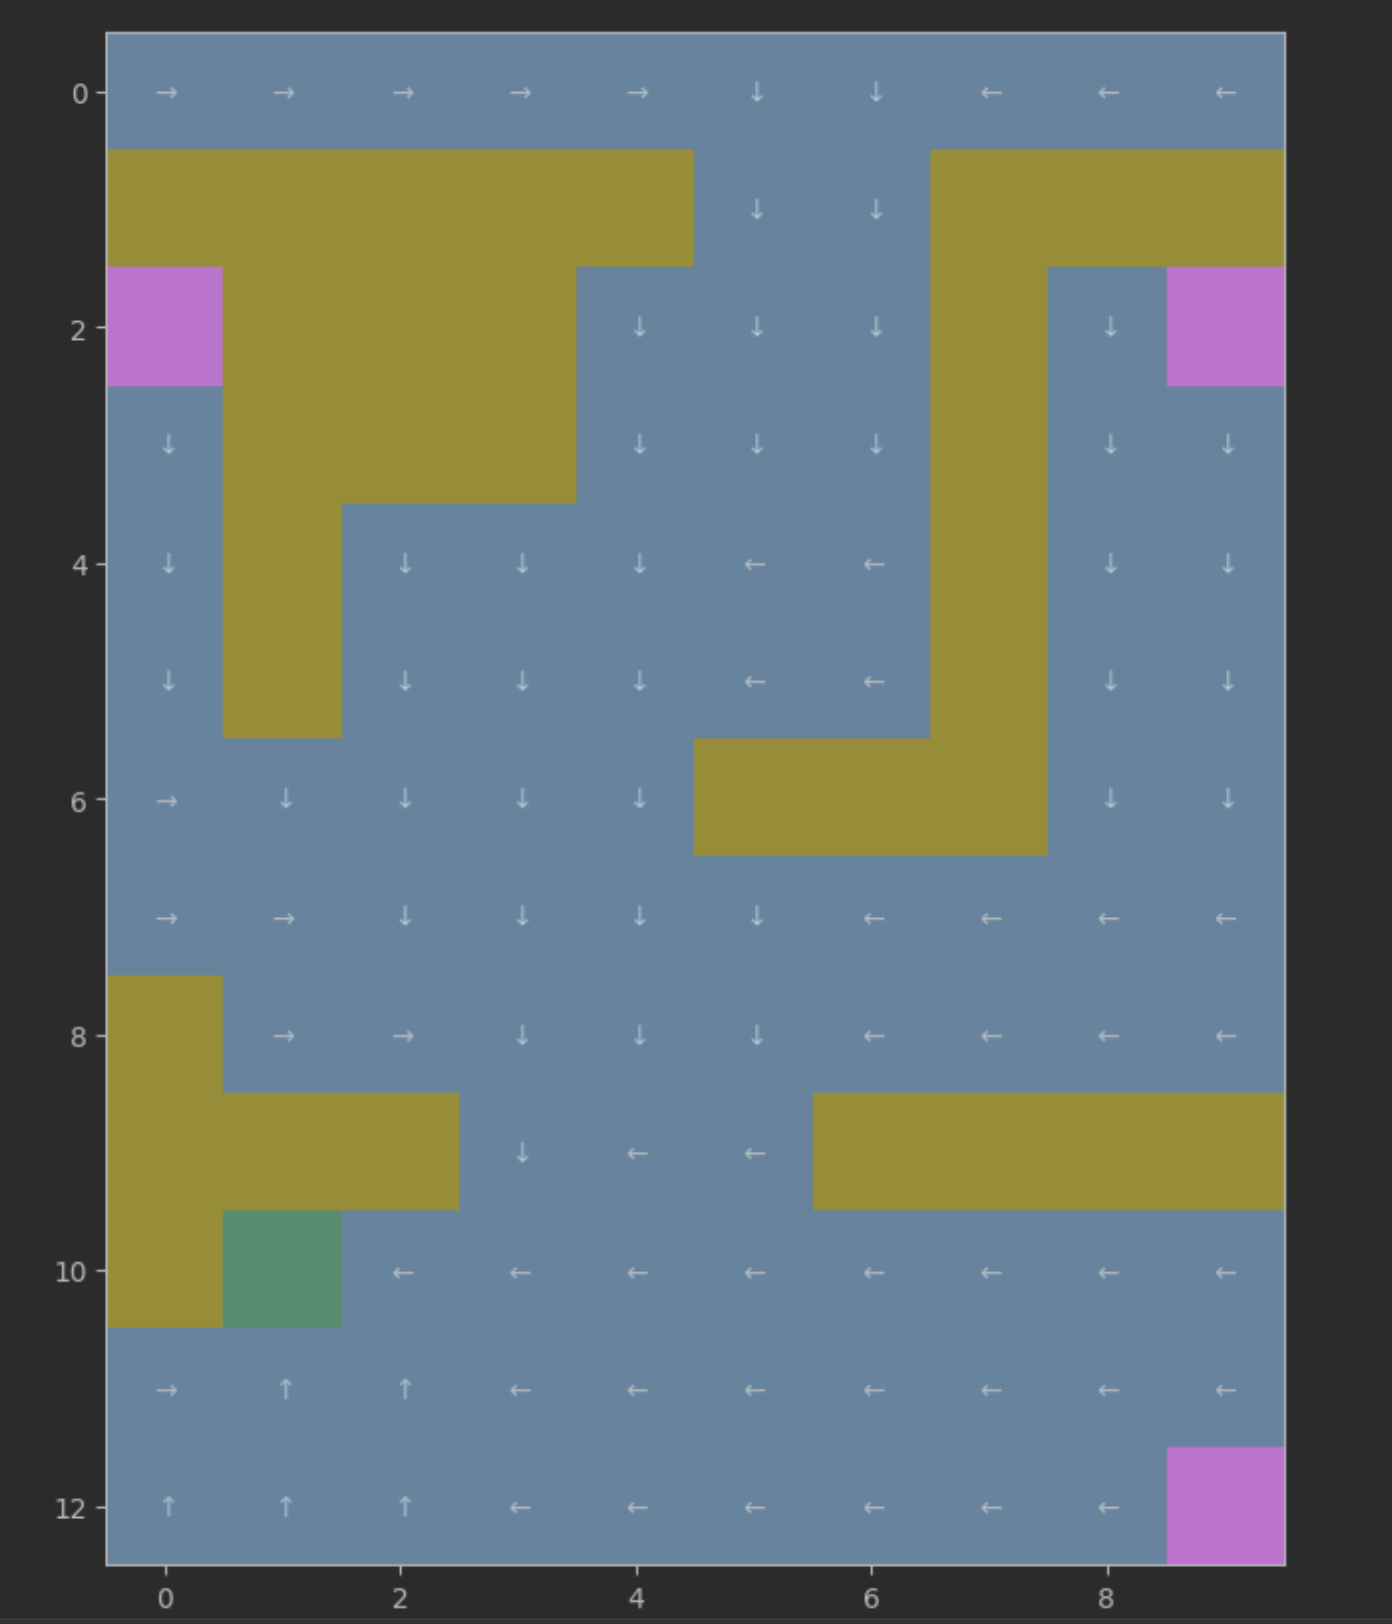
\includegraphics[width=0.9\linewidth]{images/dp_policy}
            \caption{dp policy}\label{fig:dp_policy}
        \end{subfigure}
        \begin{subfigure} {0.5\textwidth}
            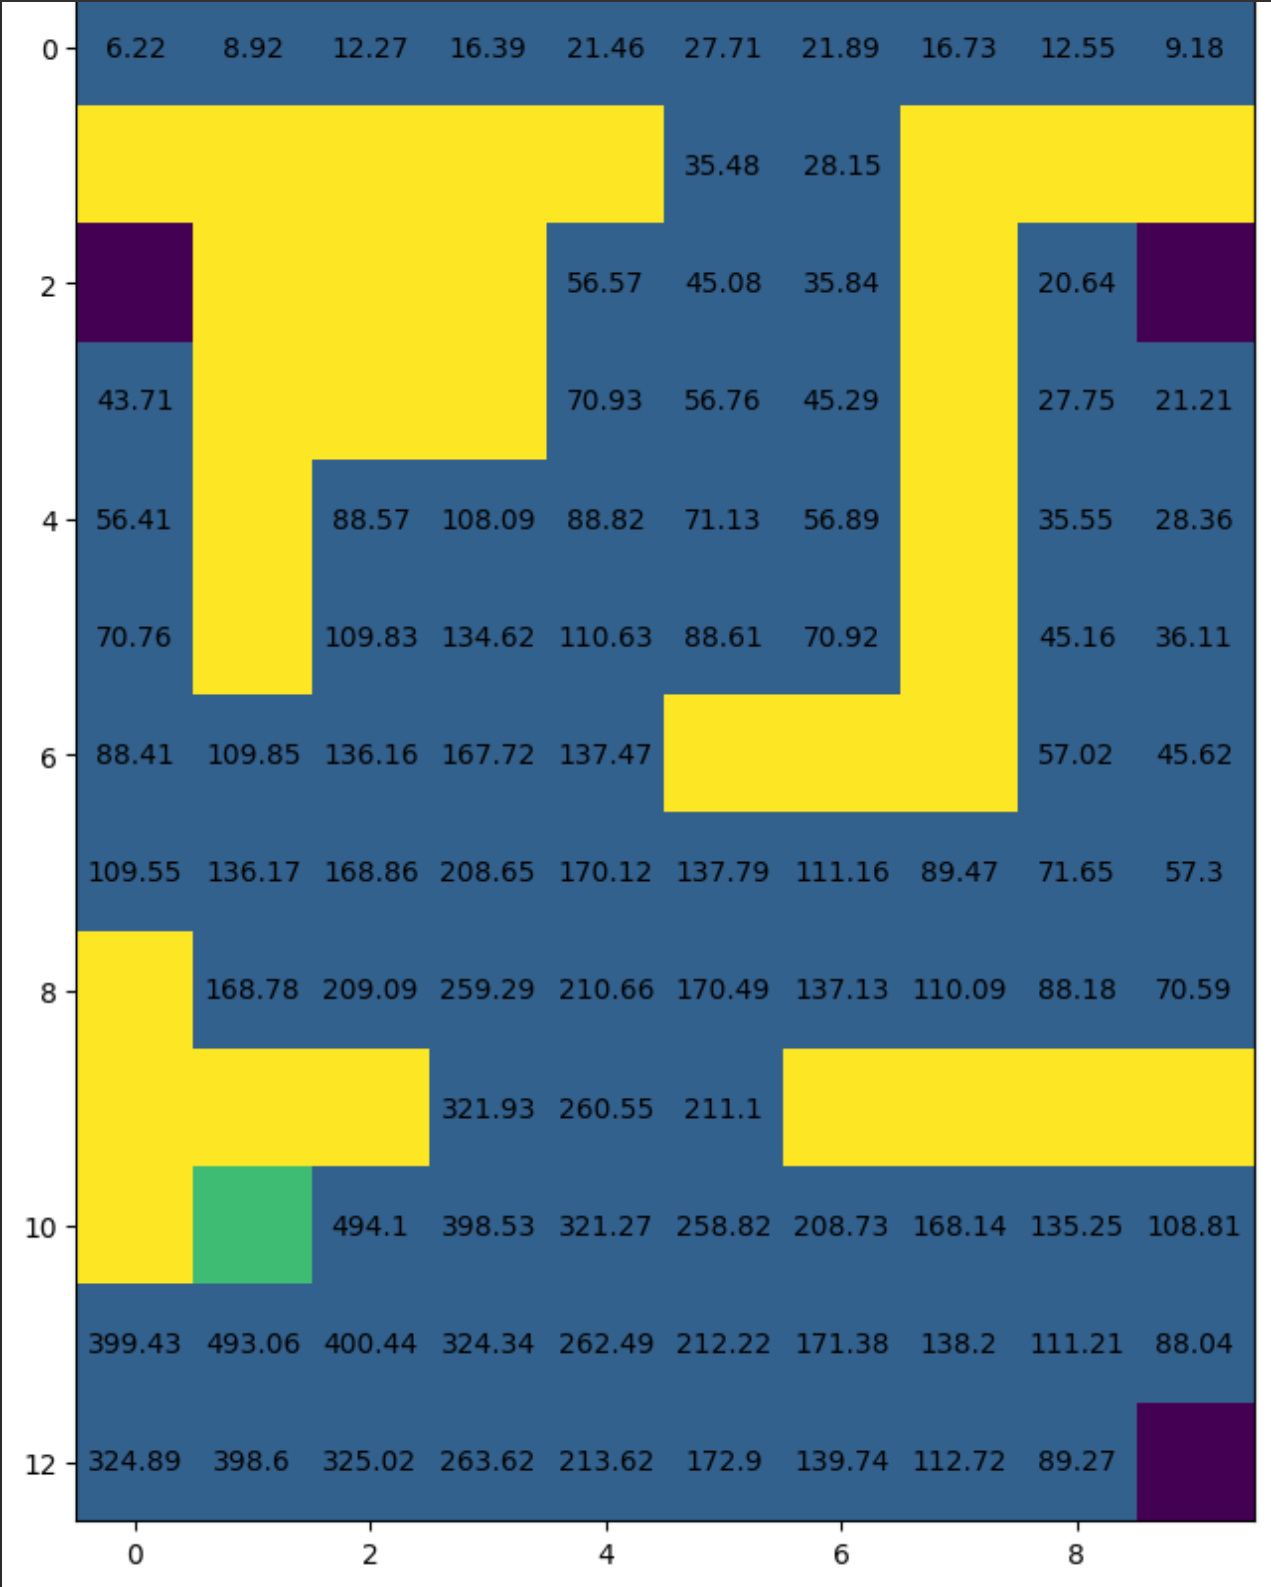
\includegraphics[width=0.9\linewidth]{images/dp_value}
            \caption{dp value}\label{fig:dp_value}
        \end{subfigure}
    \end{figure}

    \subsection{Part 3}\label{subsec:question-1-3}
    For $p < 0.25$, attempting to take the ``best'' action no longer yields the best expected return.
    Hence, the optimal policy would select any action other than the ``best'' action.
    For $p == 0.25$, attempting to take any action would yield the same expected return, as the committed action is fully random.
    The optimal policy would then be defaulted to action 0, which is going upwards.
    For $p > 0.25$, attempting to take the ``best'' action is indeed the optimal solution, as chosen by the optimal policy.

    For $\gamma < 0.5$, the state values around the goal state fall off quickly, with the rest of the states having values close to zero.
    This is likely due to that the agent is myopic and is less influenced by the goal state's value of 500.
    For $\gamma > 0.5$, the state values are more widely propagated to the rest of the board and fall off from the goal state less quickly.


    \section{Question 2}\label{sec:question-2}

    \subsection{Part 1}\label{subsec:question-2-1}
    I used an on-policy $\epsilon$-greedy first-visit MC iterative learning to control algorithm to solve the problem.

    $\epsilon$-greedy policy is used to allow for exploring the states, as the starting states are only part of the total states.
    The hyperparameter $\epsilon$ is set to 0.5 to allow for a certain degree of exploration.
    $\epsilon$ is decreasing with number of episodes to satisfy the GLIE convergence condition.

    The total number of episodes is set to 4000.
    This decision is guided by plotting total non-discounted reward vs episodes.
    \begin{figure}[h]
        \begin{subfigure} {0.5\textwidth}
            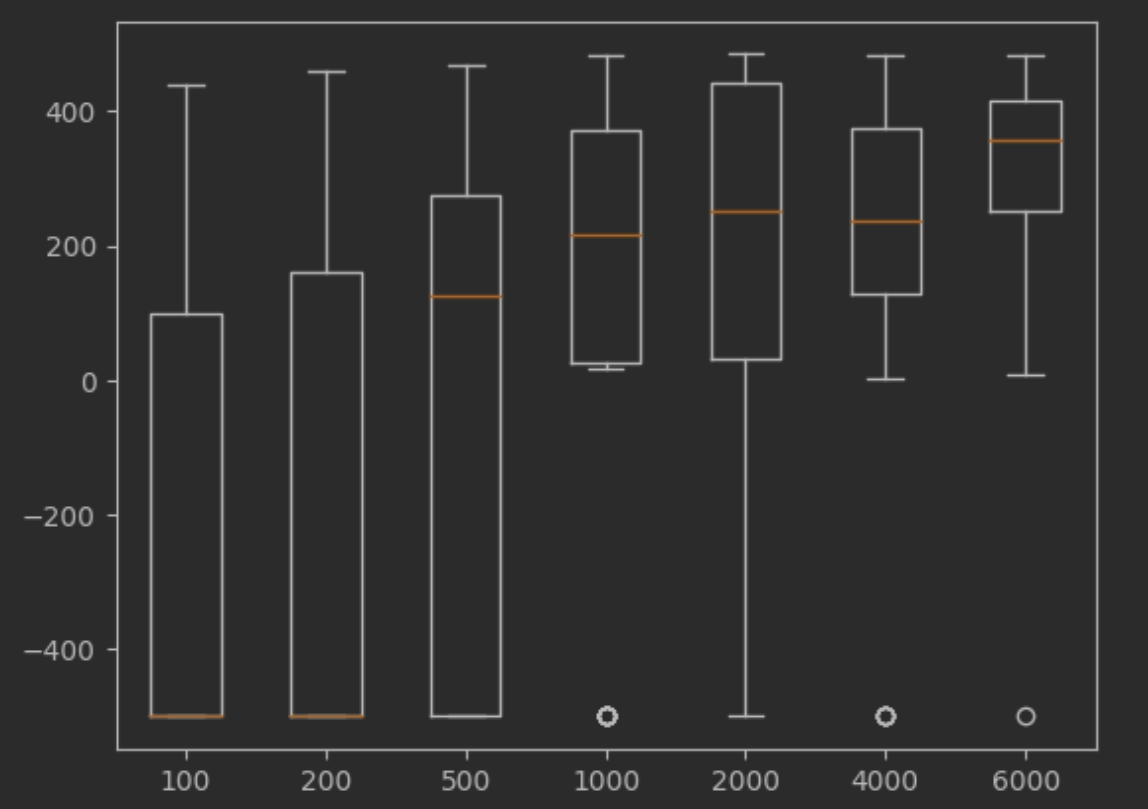
\includegraphics[width=0.9\linewidth]{images/n_episode_vs_reward_mc}
            \caption{mc return vs episodes}\label{fig:mc_return_vs_epi}
        \end{subfigure}
        \begin{subfigure} {0.5\textwidth}
            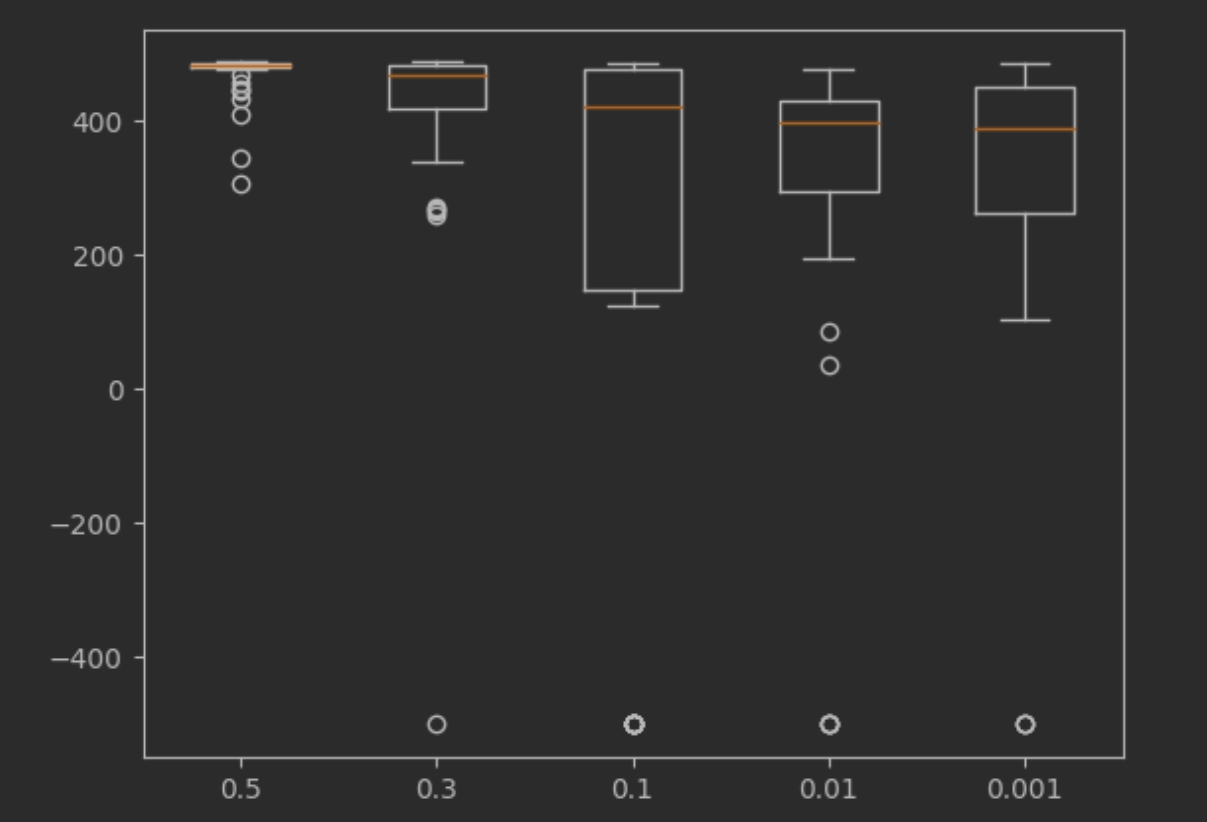
\includegraphics[width=0.9\linewidth]{images/alpha_vs_reward_mc}
            \caption{mc return vs alpha}\label{fig:mc_return_vs_alpha}
        \end{subfigure}
    \end{figure}

    The learning rate $\alpha$ is set to 0.5, as guided by experiments.

    First-visit MC is chosen for its effectiveness and simplicity.

    The assumption made about the environment is that the reward would be constant with respect to time.
    In other words, the environment would not change with time.

    \subsection{Part 2}\label{subsec:question-2-2}
    \begin{figure}[h]
        \begin{subfigure} {0.5\textwidth}
            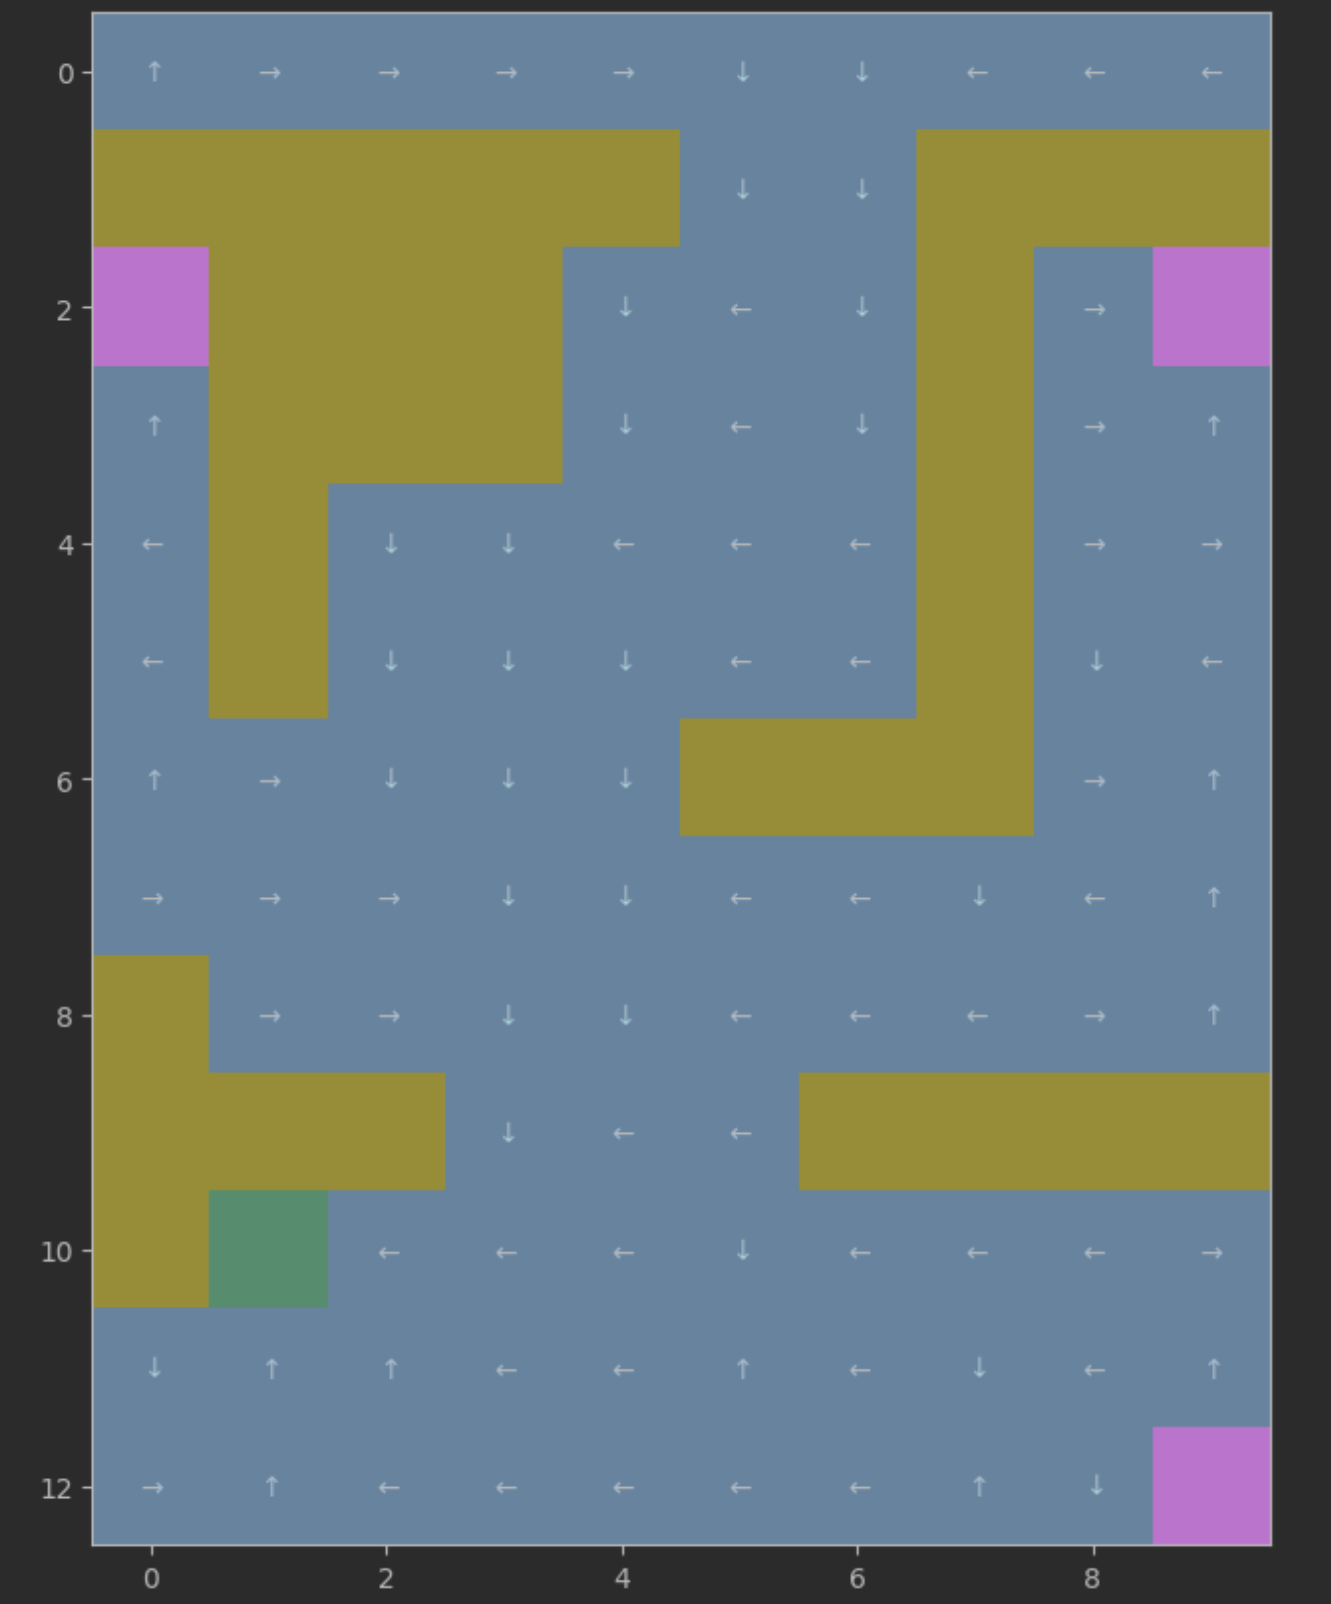
\includegraphics[width=0.9\linewidth]{images/mc_policy}
            \caption{mc policy}\label{fig:mc_policy}
        \end{subfigure}
        \begin{subfigure} {0.5\textwidth}
            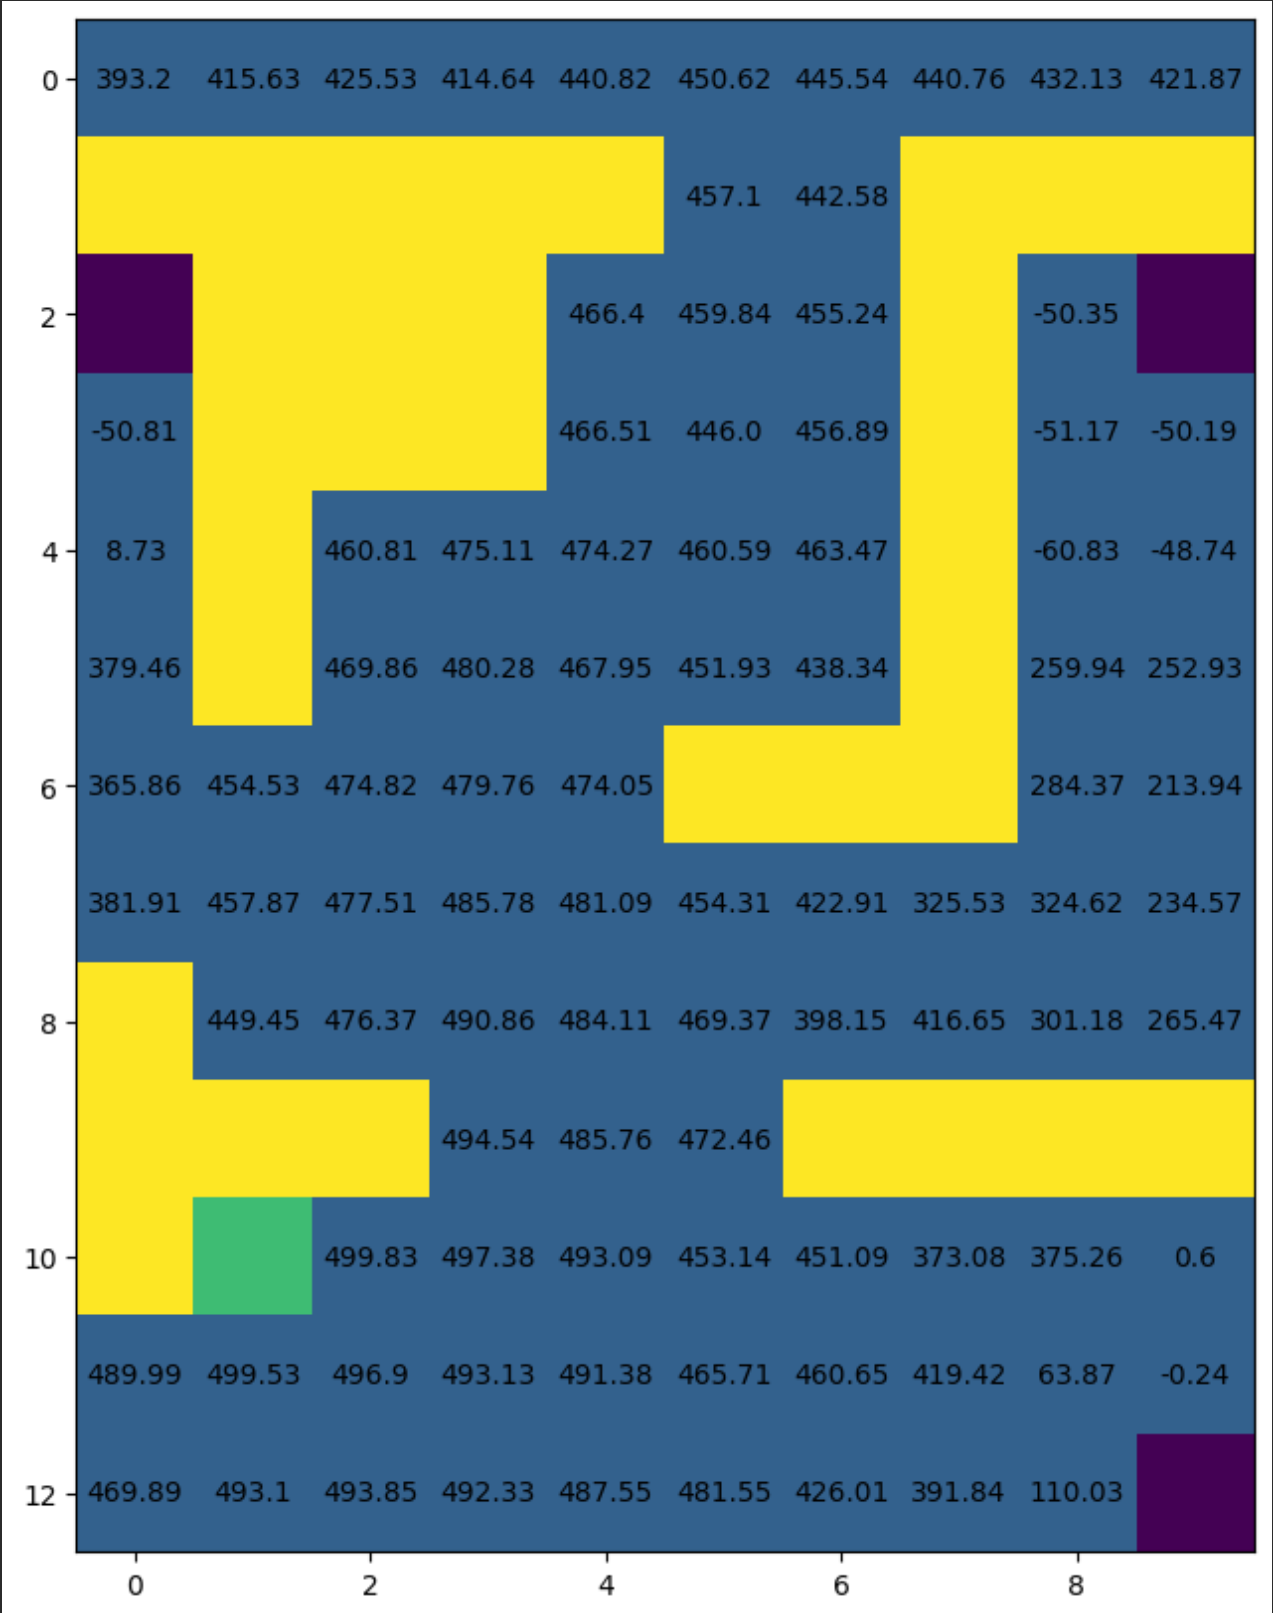
\includegraphics[width=0.9\linewidth]{images/mc_value}
            \caption{mc value}\label{fig:mc_value}
        \end{subfigure}
    \end{figure}

    \subsection{Part 3}\label{subsec:question-2-3}
    The randomness comes from the fact that actions are chosen from a set of possible actions, each assigned with some probability.
    The choice made every time can be different and random.
    To establish significance of the final learned policy, multiple runs are carried out and the distribution of final total non-discounted rewards is obtained.
    From the summary statistics of different number of runs we can conclude that 5 replications would be sufficient.
    \begin{figure}[h]
        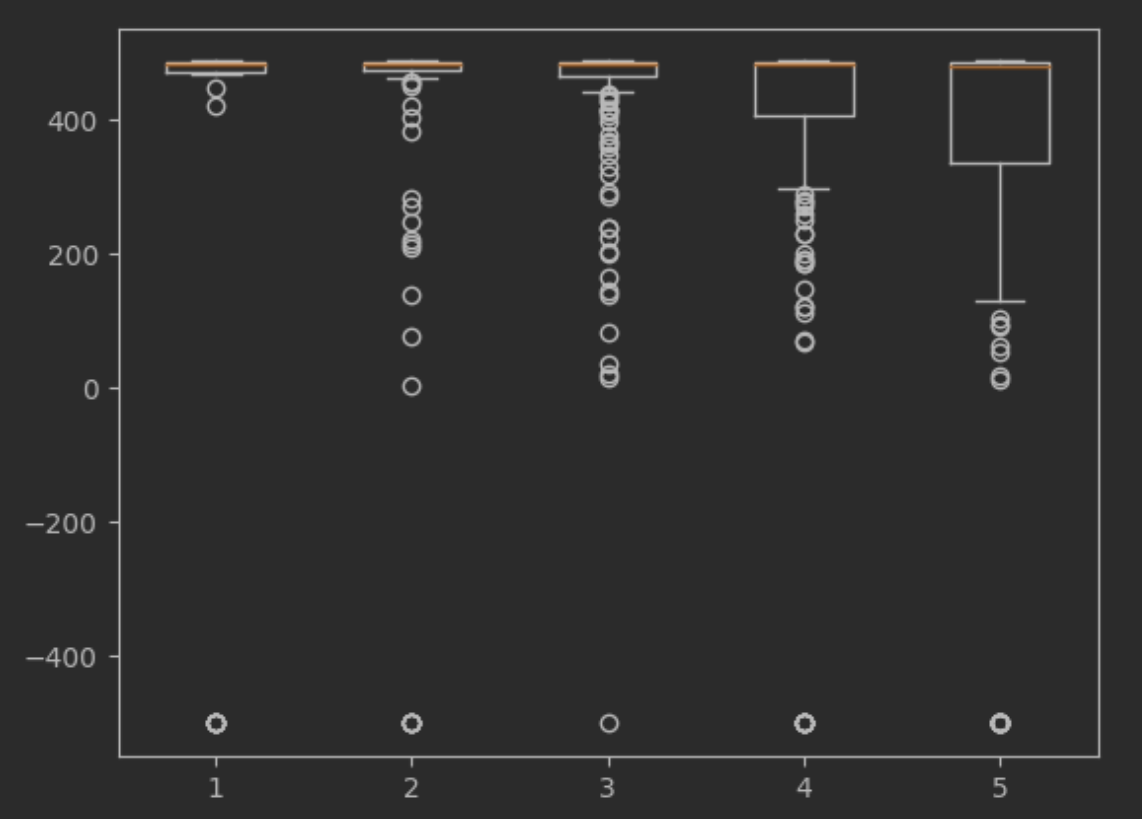
\includegraphics[width=0.9\linewidth]{images/n_replications_vs_reward_mc}
        \caption{n replications vs return (x-axis should read 5, 10, 15, 20, 25)}\label{fig:mc_replication_reward}
    \end{figure}

    \subsection{Part 4}\label{subsec:question-2-4}
    \begin{figure}[h]
        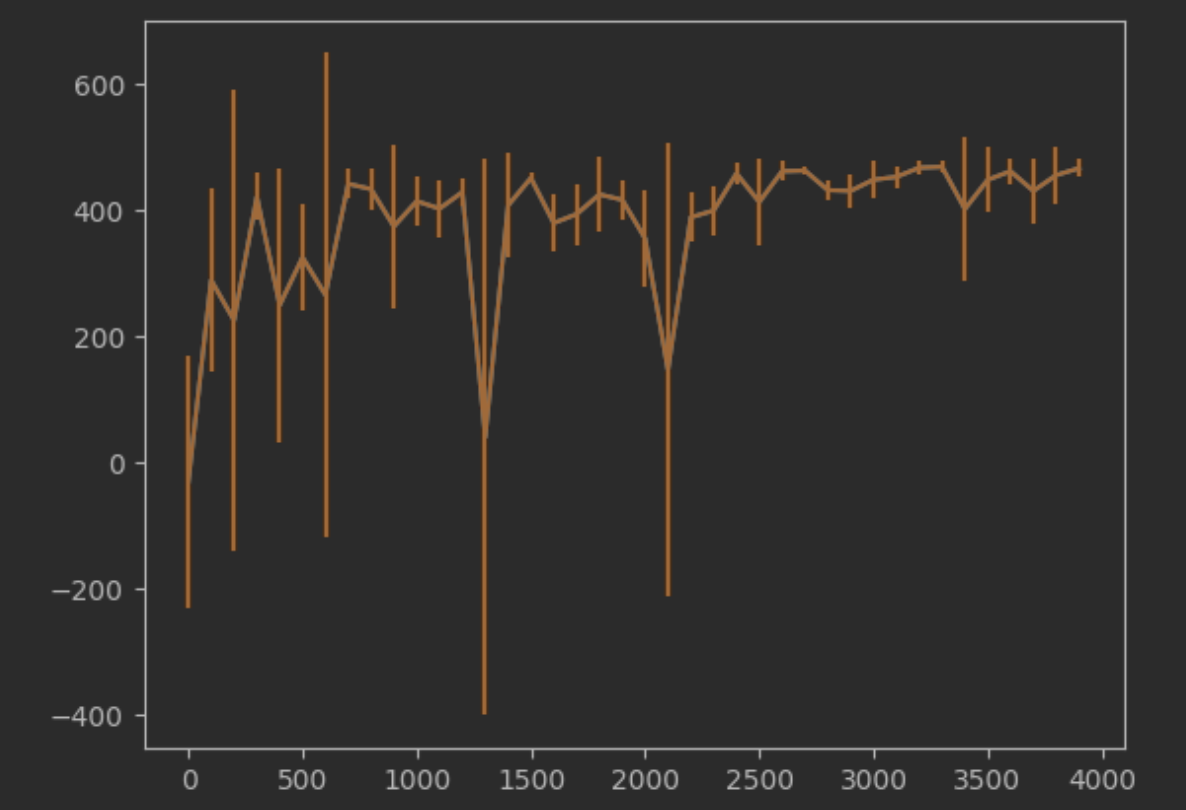
\includegraphics[width=0.9\linewidth]{images/mc_learning_curve}
        \caption{mc learning curve}\label{fig:mc_learning_curve}
    \end{figure}
    (Figure~\ref{fig:mc_learning_curve})

    \subsection{Part 5}\label{subsec:question-2-5}
    \begin{figure}[h]
        \begin{subfigure} {0.5\textwidth}
            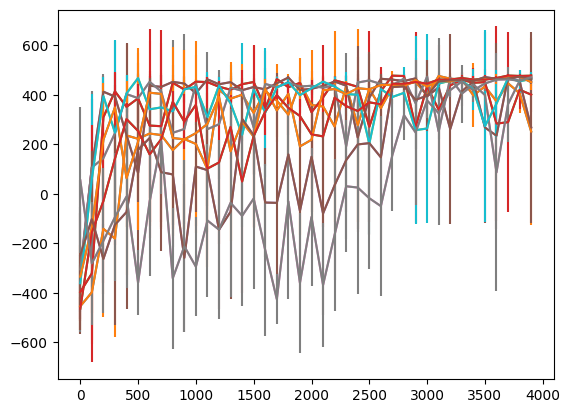
\includegraphics[width=0.9\linewidth]{images/mc_learning_curve_epsilons}
            \caption{mc learning curve for different epsilons}\label{fig:mc_learning_curve_epsilons}
        \end{subfigure}
        \begin{subfigure} {0.5\textwidth}
            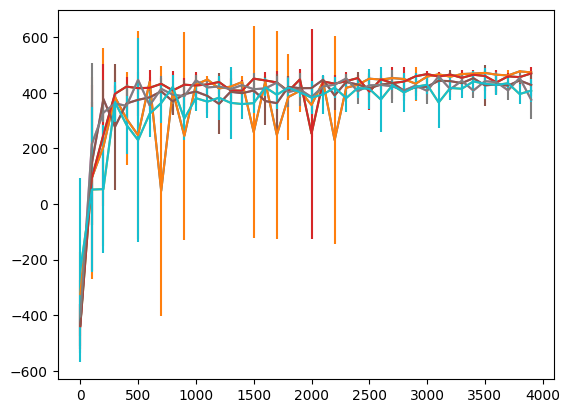
\includegraphics[width=0.9\linewidth]{images/mc_learning_curve_alphas}
            \caption{mc learning curve for different alphas}\label{fig:mc_learning_curve_alphas}
        \end{subfigure}
    \end{figure}
    For different $\epsilon$, the learning curve is more stable for a smaller $\epsilon$.
    Although the $\epsilon$ would tend to zero to satisfy GLIE, smalelr $\epsilon$ makes learning from successful episodes easier.

    For different $\alpha$, the learning converges in a similar manner.
    This is because that the environment is stationary, hence $\alpha$ values does not influence the learning much.
    The older episodes are as useful as the latest episodes.


    \section{Question 3}\label{sec:question-3}

    \subsection{Part 1}\label{subsec:question-3-1}
    I used an on-policy TD learning to control algorithm to solve the problem.
    The learning rate $\alpha$ is set to 1e-2 and decreasing with respect to t to allow for convergence.
    The choice of actions follows $\epsilon$-greedy with a decreasing $\epsilon$ from initial value 0.5 to satisfy GLIE.
    The assumption made is that the environment is stationary.

    \subsection{Part 2}\label{subsec:question-3-2}
    \begin{figure}[h]
        \begin{subfigure} {0.5\textwidth}
            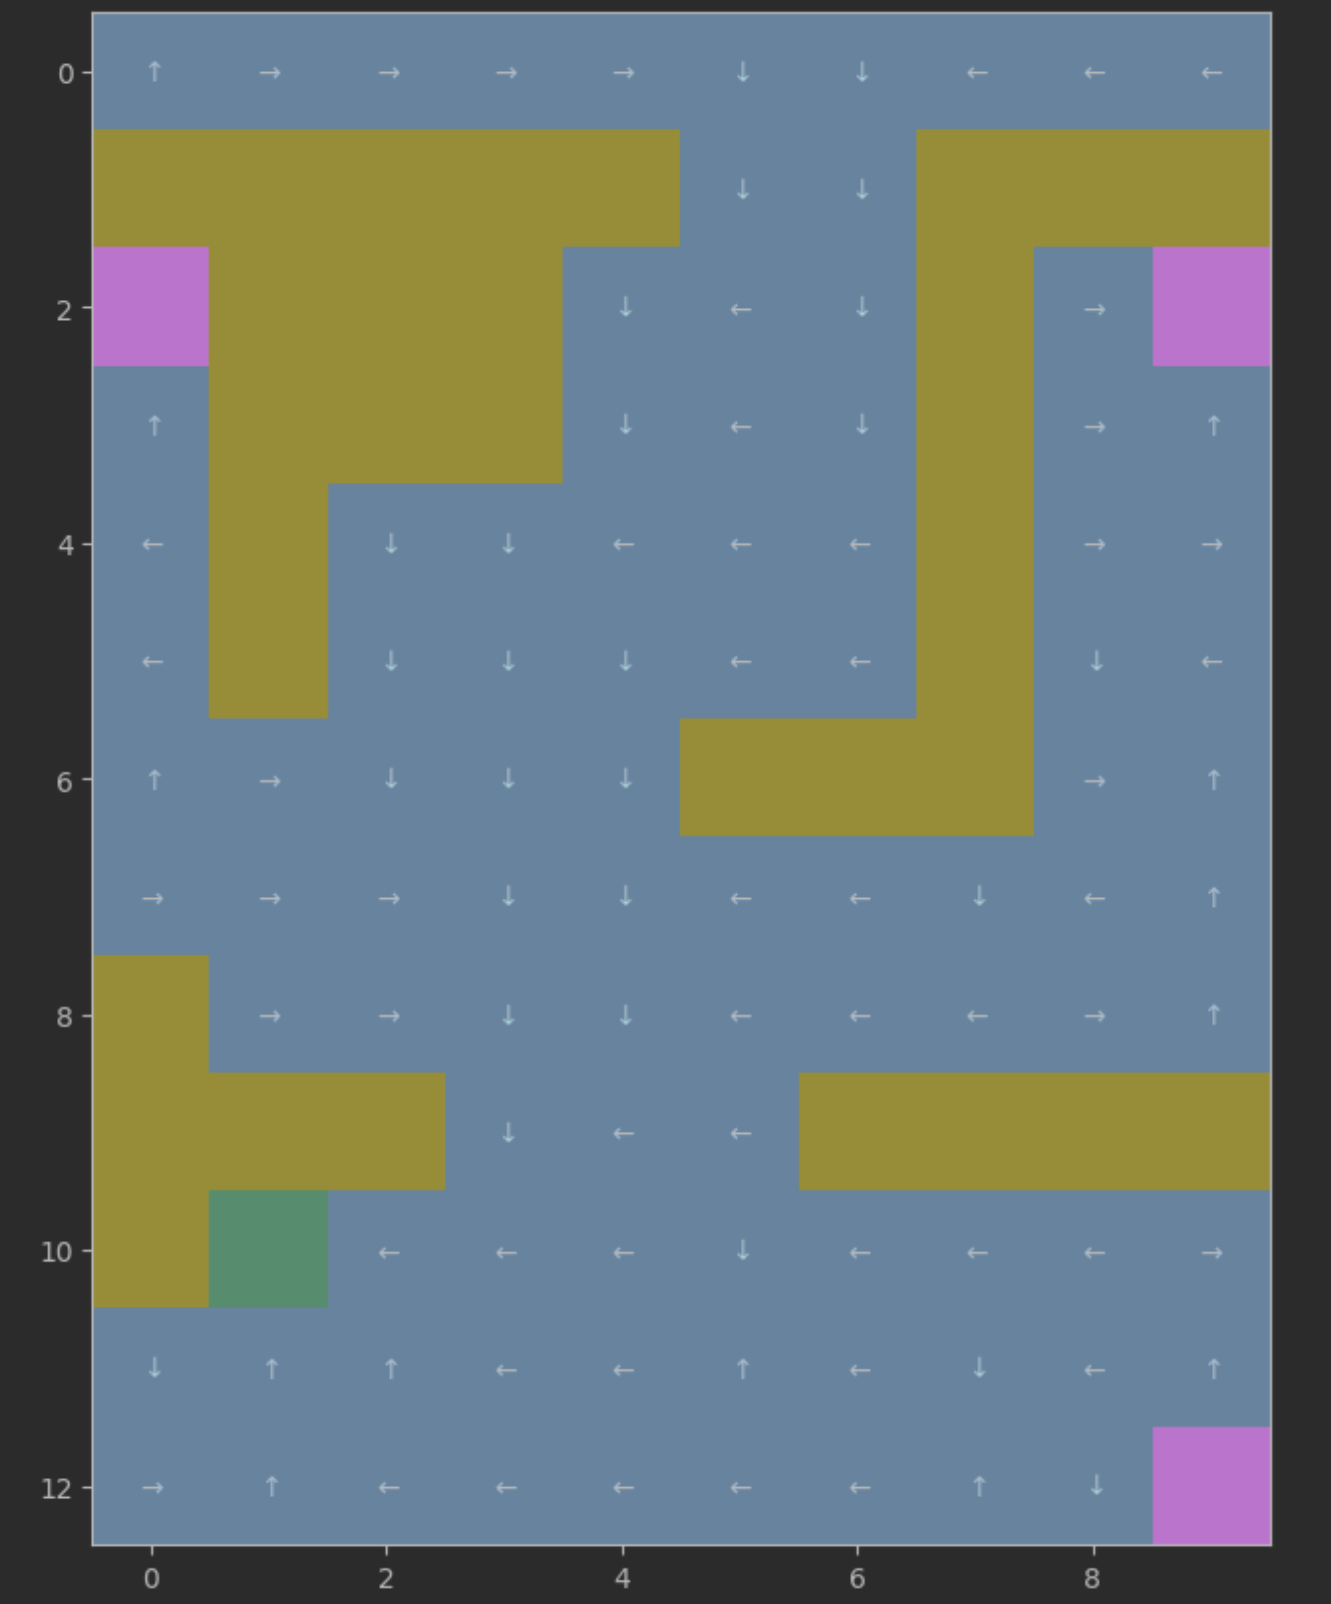
\includegraphics[width=0.9\linewidth]{images/mc_policy}
            \caption{td policy}\label{fig:td_policy}
        \end{subfigure}
        \begin{subfigure} {0.5\textwidth}
            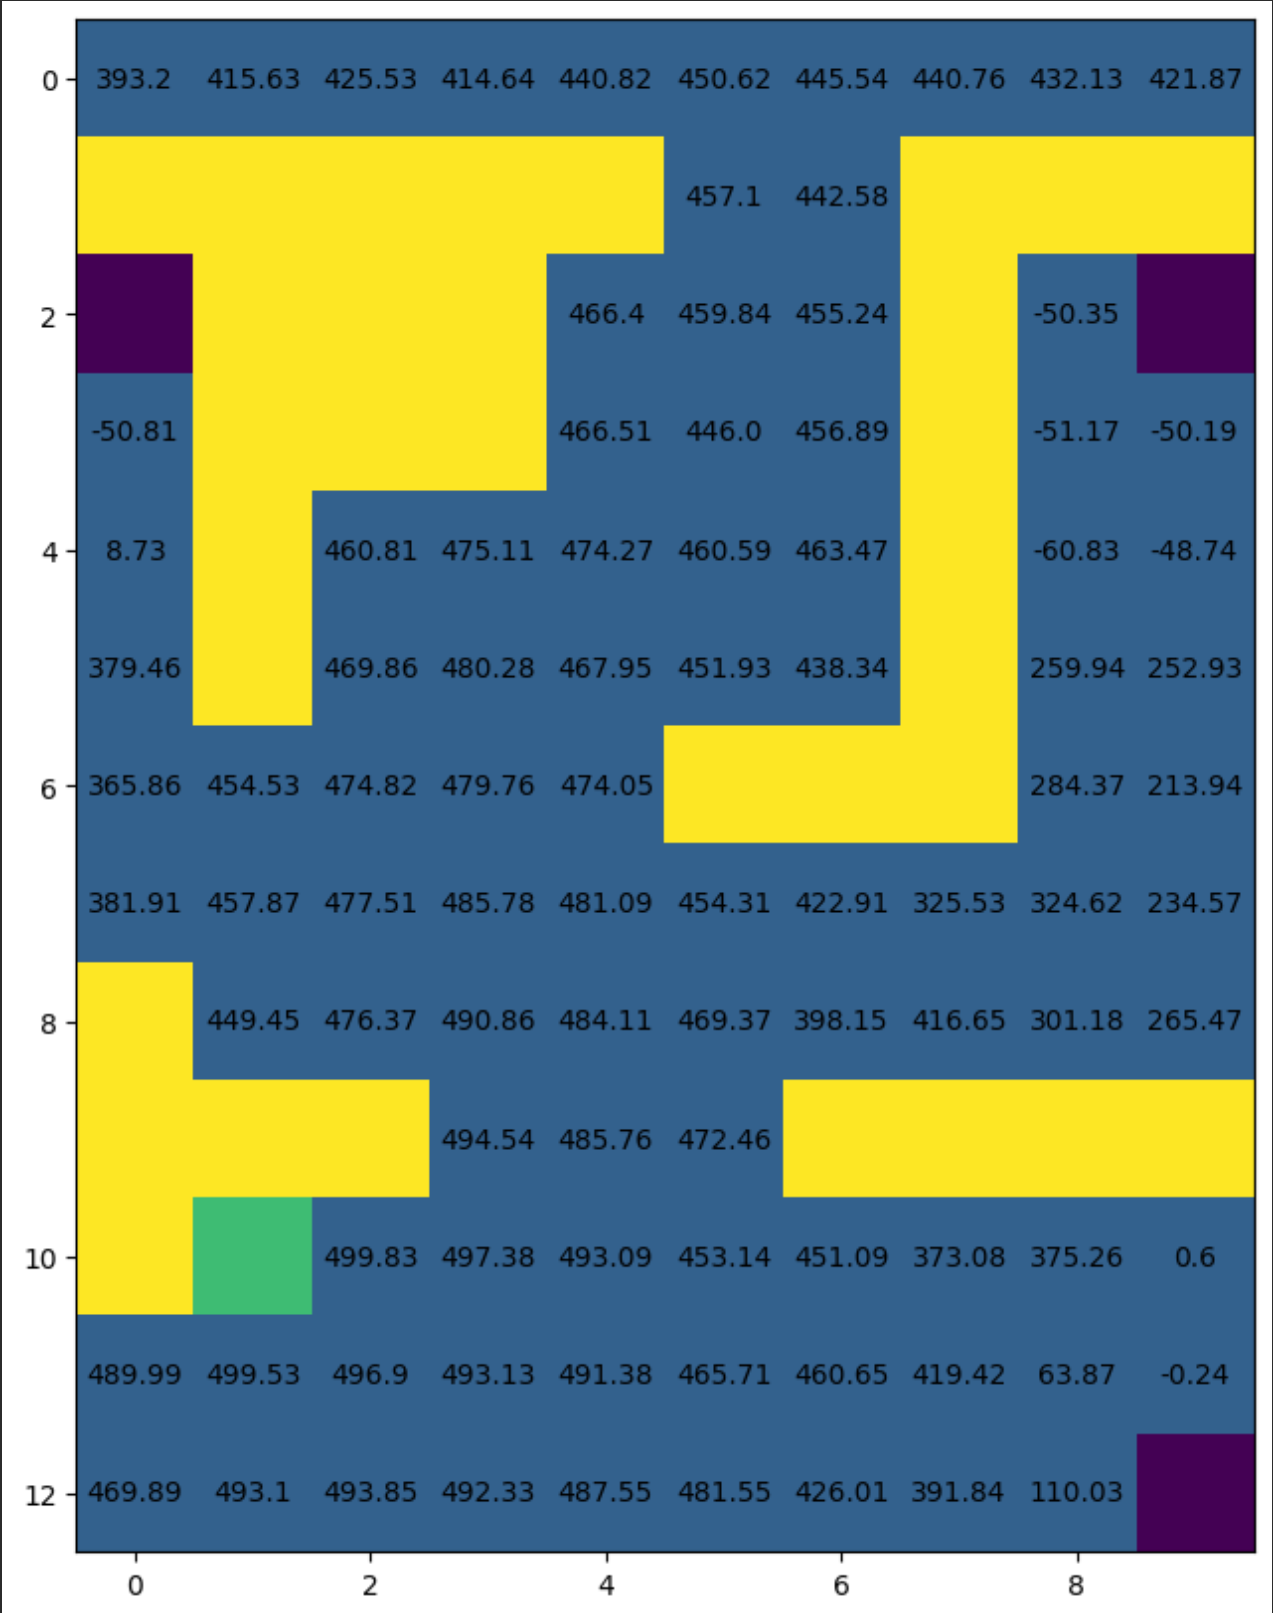
\includegraphics[width=0.9\linewidth]{images/mc_value}
            \caption{td value}\label{fig:td_value}
        \end{subfigure}
    \end{figure}

    \subsection{Part 3}\label{subsec:question-3-3}
    learning curve
    TODO

    \subsection{Part 4}\label{subsec:question-3-4}
    learning curve
    varying $\epsilon$
    varying $\alpha$
    TODO


    \section{Question 4}\label{sec:question-4}

    \subsection{Part 1}\label{subsec:question-4-1}

\end{document}
